\documentclass[12pt,a4paper]{article}
\usepackage{graphicx}
\usepackage{amsmath}
\usepackage{amssymb}
\usepackage{subfigure}
\usepackage{booktabs}
\usepackage{color}
\usepackage{listings}
\usepackage{eurosym}
\usepackage{mathtools} % for \mydef
\usepackage{float}
\usepackage{natbib}
\usepackage{gensymb} % for \degree
%\usepackage{authblk} % for multiple authors with different affiliations
\usepackage[small]{titlesec}
\usepackage[displaymath, mathlines]{lineno}

% see http://tex.stackexchange.com/questions/99316/symbol-for-external-links
\usepackage{fontawesome}
\usepackage[hidelinks]{hyperref}
% Redefinition, symbol included in link:
\let\orighref\href
\renewcommand{\href}[2]{\underline{\orighref{#1}{#2}}}
% hyphens option for hyperref: enables line-breaks at hyphens. Otherwise only at slashes /. Ugly
%\PassOptionsToPackage{hyphens}{url}\usepackage{hyperref}

\addtolength{\oddsidemargin}{-2cm}
\addtolength{\evensidemargin}{-2cm}
\addtolength{\textwidth}{4cm}
\addtolength{\topmargin}{-2cm}
\addtolength{\textheight}{2cm}

%%%%%%%%%%%%%%%%%%%%%%%%%%%%%%%%%%%%%%%%%%%%%%%%
% REMOVE FOR FINAL VERSION


%%DRAFT HEADERS on normal pages
%\usepackage{fancyhdr}
%\pagestyle{fancy}
%\fancyhf{} % clear all headers and footers
%\fancyhead[C]{{\bf DRAFT}}
%\cfoot{\thepage}
%%DRAFT HEADERS on TOC and Chapter pages
%\fancypagestyle{plain}{
%	\fancyhf{}
%	\fancyhead[C]{{\bf DRAFT}}
%	\cfoot{\thepage}
%}
%%DRAFT HEADERS on title pages
%\fancypagestyle{empty}{
%	\fancyhf{}
%	\fancyhead[C]{{\bf DRAFT}}
%}

%%%%%%%%%%%%%%%%%%%%%%%%%%%%%%%%%%%%%%%%%%%%%%%%%%%%%%%%


\renewcommand{\familydefault}{\sfdefault}

\graphicspath{{../figures_pdf/}} 

%\linenumbers

\title{
	{\bf DRAFT}\\
	Notes on running ROMS on Amazon Web Services 
}

\author{Stefan Riha\thanks{Email: stefan@sriha.net}}
%\date{}

\begin{document}
	\setlength{\parindent}{0cm}
	\maketitle

\section{Preliminary results}
	All results shown were produced with ROMS \citep{shchepetkin2005regional}, compiled with Open MPI using gfortran.
	
	\begin{figure}[H]
		\centering
		\includegraphics[width=0.5\textwidth]{met_t2micro.pdf}
		\caption{Time (in seconds) spent per process for the ROMS "small" benchmark test (benchmark1.in), as function of the number of processes. Computations are performed on t2.micro instances of AWS, which have one vCPU per (virtual) node (2016/11/01). Each data point shows the average over all processes, measured from one single experiment. The inset shows the domain partition (tiling) of the 512x64(x30) point domain. The result suggests that partitioning along the first dimension yields better performance.}
		\label{fig:met_t2micro}
	\end{figure}

	\begin{figure}[H]
	\centering
	\includegraphics[width=0.5\textwidth]{met_c4large.pdf}
	\caption{Same as Fig. \ref{fig:met_t2micro}, but computations are performed on c4.large instances of AWS, which have 2 vCPUs per (virtual) node. In the case of c4 instances, a vCPU is defined as a single thread of a custom 2.9 GHz Intel Xeon E5-2666 v3 (Haswell) processor (2016/11/01).}
	\label{fig:met_c4large}
\end{figure}

\begin{figure}[H]
	\centering
	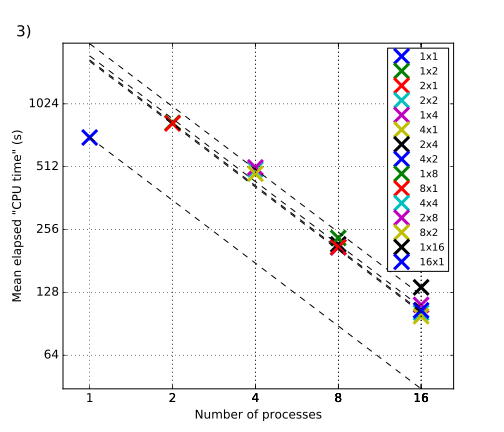
\includegraphics[width=0.5\textwidth]{met_c44xlarge.pdf}
	\caption{Time (in seconds) spent per process for the ROMS "medium" benchmark test (benchmark2.in), as function of the number of processes. Computations are performed on c4.4xlarge instances of AWS, which have 16 vCPUs per (virtual) node.}
	\label{fig:met_c4large}
\end{figure}

\subsection{Computational and monetary costs of a realistic study}

The preliminary test above allow a rough estimate of the computational and monetary costs involved in a realistic study. By monetary cost we mean the financial cost of renting AWS' hardware to conduct a study of a given computational cost. As an example we consider \cite{kumar2015midshelf}, who validate the midshelf and surfzone circulation generated by a numerical model against observations.  They use a coupled ROMS-SWAN model and compare it to observations from the 2006 Huntington Beach (San Pedro Bay, California, U.S.A.) experiment. We assume that such studies, which investigate the transport processes directly adjacent to the coast, are particularly important for commercial applications. Whether or not it is actually \emph{technically feasible} to conduct such a highly complex state-of-the-art simulation on AWS' cloud infrastructure, is not shown here. Instead, the objective here is to gain a (very rough) order-of-magnitude estimate of the involved cost, \emph{assuming} technical feasibility. 

The numerical experiment of \cite{kumar2015midshelf} consists of the following components:

\begin{itemize}
	\item Wind forcing
	\item Wave forcing
	\item Tide forcing
	\item Buoyancy forcing
\end{itemize}

which are coupled by the open-source Coupled Ocean-Atmosphere-Wave-Sediment (COAWST) Transport model \citep{warner2008using,web:coawst}, which couples an atmospheric (Weather Research and Forecasting model, WRF), wave (SWAN), three-dimensional circulation and stratification (ROMS) and sediment transport models. COAWST is integrated by the Model Coupling Toolkit (MCT, \citealt{web:mct}) to exchange data fields between the models. They use the following nested grids:

\begin{itemize}
	\item U.S. West Coast and eastern Pacific (L0):  $\Delta=5\,\rm km$, area $4000\times3000\,\rm km^2$ ($800\times600$ grid points)
	\item Southern California Bight (L1):  $\Delta=1\,\rm km$, area $800\times700\,\rm km^2$ ($800\times700$ grid points)
	\item Interior bight region (L2): $\Delta=250\,\rm m$, area $500\times300\,\rm km^2$ ($2000\times1200$ grid points)
	\item San Pedro Bay (L3): $\Delta=75\,\rm m$, area $80\times70\,\rm km^2$ ($1067\times934$ grid points)
\end{itemize}

\subsection{TODO}

\begin{itemize}
	\item Relate monetary cost of computations to cost of labor.
\end{itemize}

	
\bibliography{main.bib}
\bibliographystyle{model2-names}

\end{document}

 
